%! Author = Kevin
%! Date = 29.07.2022

% Preamble
\documentclass{acm_proc_article-sp}

% Packages
\usepackage{graphicx}
\graphicspath{images/}
\usepackage{epstopdf}
\usepackage{xr-hyper}
\usepackage{hyperref}
\usepackage{todonotes}
\usepackage[nodayofweek]{datetime}
\usepackage{acronym}
\usepackage{multirow}
\usepackage{colortbl}
\usepackage{listings-rust}






\usepackage{subfiles}

\definecolor{lightgray}{rgb}{.9,.9,.9}
\definecolor{darkgray}{rgb}{.4,.4,.4}
\definecolor{purple}{rgb}{0.65, 0.12, 0.82}

\lstdefinelanguage{JavaScript}{
    keywords={typeof, new, true, false, catch, function, return, null, catch, switch, var, if, in, while, do, else, case, break, const},
    keywordstyle=\color{blue}\bfseries,
    ndkeywords={class, export, boolean, throw, implements, import, this, require},
    ndkeywordstyle=\color{darkgray}\bfseries,
    identifierstyle=\color{black},
    sensitive=false,
    comment=[l]{//},
    morecomment=[s]{/*}{*/},
    commentstyle=\color{purple}\ttfamily,
    stringstyle=\color{red}\ttfamily,
    morestring=[b]',
    morestring=[b]"
}

\lstset{
    language=JavaScript,
    backgroundcolor=\color{lightgray},
    extendedchars=true,
    basicstyle=\footnotesize\ttfamily,
    showstringspaces=false,
    showspaces=false,
    numbers=left,
    numberstyle=\footnotesize,
    numbersep=9pt,
    tabsize=2,
    breaklines=true,
    showtabs=false,
    captionpos=b
}


% Commands
\newdate{dateAtomShell}{15}{07}{2013}
\newdate{dateRenameElectron}{23}{04}{2015}
\newdate{dateTauriRelease}{31}{12}{2019}
\date{\displaydate{date}}
\pagenumbering{arabic}
\newcommand{\secref}[1]{\autoref{#1}.~\nameref{#1}}
\newcommand\figref{Figure~\ref}
\newcommand{\shellcmd}[1]{\\\indent\indent\texttt{\footnotesize\# #1}\\}

% Document
\begin{document}

    \title{{\ttlit Electron} and {\ttlit Tauri}: Comparison of web-frameworks for building cross-platform desktop applications}
    \numberofauthors{1}
    \author{
        \alignauthor
        Kevin L\"uttge \\
        %\titlenote{Dr.~Trovato insisted his name be first.}\\
        \affaddr{University of Kassel}\\
        %\affaddr{Software Engineering Research Group}\\
        %\affaddr{Department of Computer Science and Electrical Engineering}\\
        %\affaddr{Wilhelmsh\"oher Allee 73, 34121 Kassel, Germany}\\
        %\email{trovato@corporation.com}
    }

    \maketitle

    \begin{abstract}
        Web-frameworks like Electron provide the possibility to easily develop cross-platform desktop applications by using common web-technologies
        such as \ac{HTML}, \ac{CSS} and JavaScript.
        The increasing popularity of those frameworks is shown by various day-to-day applications namely WhatsApp, Discord or Visual Studio Code
        that are built with Electron.
        Two years ago Tauri came up, whose developers claimed it ``to be faster, smaller and more focused on security than other alternative frameworks``~\cite{tauri}.
        This paper will discuss the differences and similarities between Electron and Tauri, in terms like architecture, performance or security.
        Therefor a counter application is implemented for each framework to analyze and compare the development process.
    \end{abstract}
    %Introduction checked
    \section{Introduction}\label{sec:introduction}
Cross-platform web-frameworks like Electron, Tauri or Flutter provide the possibility of using standard web-technologies like \ac{HTML}, \ac{CSS} and JavaScript or entire web-frameworks
like Angular to develop or migrate classic desktop applications to web applications.
The traditional approach of implementing desktop applications needs the developer to consider different \ac{API} or environments of the major operating systems \ac{OS}
Windows, Mac and Linux.
In fact each application has to be implemented multiple times to adapt \ac{OS}-specific requirements and produces redundant code.
In context of consumer applications the usage of such frameworks like Electron allows companies and product owners to develop new target groups, but also increases the pool of potential applicants,
since they provide web developers technologies and features to implement desktop applications without the knowledge of standard programming languages that are used for desktop applications
like C/C++ or Java.
But also institutions or universities and their students benefit of it, because due to the fact of cross-platform capabilities, applications can be used by many devices and decrease costs
since they do not need particular hardware to be executed.

\subsection{Background}\label{subsec:background}
Over the past years web-frameworks for building desktop applications have experienced more and more attention, which can be expressed by the number of articles related to such topics or the temporal progression of Google Trends related to this topic.
This is owed to the fact of fundamental advances at web technologies like TypeScript as an improvement of JavaScript or Frontend Frameworks like Angular or React~\cite{pernice:icalepcs2019-wempr006},
which lead to a wider use of such technologies for various scenarios.
A lot of every day applications used by computer scientists like Visual Studio Code or GitHub Desktop, but also applications with usage spread over industry sectors
like Microsoft Teams, Skype or Discord and even Social Media applications like WhatsApp or Twitch are implemented using cross-platform web-frameworks.
The trend of using those applications has even grow up since the outbreak of SARS-CoV-2 in early 2020~\cite{Gorbalenya2020} and the increased number of employees working from home
as a result of lockdowns all over the world.
This lead to an increasing number of cross-platform web-frameworks with different approaches in context of building, security or performance to provide a fast and simple way even for small development teams
to use web-technologies for implementing desktop applications, since their cross-platform capabilities prevent the redundant implementation of the same application for different operating systems.

%Research Questions%
\subsection{Motivation}\label{subsec:motivation}
As mentioned in Chapter~\ref{subsec:background} various cross-platform web-frameworks came up using different technologies or languages for their backend and frontend core.
One of the oldest and most commonly used frameworks is Electron, which is backed up by several popular applications implemented with Electron like Visual Studio Code, Discord or Twitch.
Therefore, Electron has become a standard in context of cross-platform development of desktop applications and almost every new framework invented is benchmarked against it like~\cite{flutter} or~\cite{electron-javafx} or~\cite{electron-nwjs}.
Two years ago a new framework called Tauri was introduced, based on the discontent with Electrons high memory consumption or insecurity by its developers.
It was designed to improve several aspects of Electron especially in case of performance, memory usage and security~\cite{tauri}.
Since these statements are made by the developers and thus may be subjective, this paper aims to provide an objective overview to the reader of both frameworks Electron and Tauri.
Therefore, fundamental architecture as well as the frontend and backend core of each framework is explained in detail at chapter~\ref{sec:electron} for Electron and at chapter~\ref{sec:tauri} for Tauri.
This technological knowledge is applied by implementing a basic application which will be described in detail at chapter~\ref{sec:implementation} and analyzes different aspects of both.
To obtain an objective statement of the advantages and disadvantages of each framework chapter~\ref{sec:summary} compares the results of previous chapters
to isolate advantages and disadvantages to the reader.
At the end of this paper the results of previous chapters are contrasted against the statement of the Tauri developers in~\cite{tauri} and being discussed to obtain an objective
comparison.

\subsection{Related Work}\label{subsec:related-work}
An exploratory study of~\cite{explorationstudy} has worked out, that applications developed with cross-platform web-frameworks are made for various kinds of usage.
The authors also empirically documented that those frameworks are mostly used by developer teams with a median size of 1, which is a direct result of the
amount resources classical desktop development consumes.
Nevertheless, they also discovered disadvantages like a high number of used libraries due to the fact of compensating lack of features provided by web-frameworks,
but also a high ratio of platform-related issues to all issues of 20\%.

The increasing popularity of using web-technologies has been shown by~\cite{pernice:icalepcs2019-wempr006}.
Since they identified their native Java Swing desktop application as a bottleneck, the authors decided to replace it with a technology stack providing long term sustainability.
Therefore, they used several web-technologies like AngularJS or Typescript to implement ``a web-based tool for configuring experiments on the National Ignition Factory``~\cite{pernice:icalepcs2019-wempr006}.
But they also came in touch with typical problems of the JavaScript ecosystem like exit or replacement of widely used technologies bringing them to be forced to migrate from
AngularJS to its successor Angular.
It has to be mentioned that the authors emphasized the community support especially in case of migration by providing tools for those cases.

Electron as a standard benchmark for cross-platform web-frameworks is shown by~\cite{electron-javafx} or~\cite{flutter}.
Both authors compared different web-frameworks against Electron.
Although the benchmark of the authors of~\cite{electron-javafx} was made with different \ac{IDE}s and the comparison between Flutter and Electron by~\cite{flutter} was based on beta version of Flutter
both found out that at the one hand Electron has better performance in case of execution time and CPU consumption and on the other that it provides more features than the compared frameworks.


    %Electron checked
    \section{Electron}
\label{sec:electron}
Electron originally was released as Atom Shell by GitHub at \displaydate{dateAtomShell}~\cite{githubReleaseV010} and downloaded approx. $83\,000\,000$ times\footnote{According to \url{https://npm-stat.com/charts.html?package=electron&from=2013-07-13&to=2022-07-30}}
The intention of the developers was ``to handle the Chromium/Node.js event loop integration and native\\APIs``~\cite{sawicki_2015} for the Atom Editor.
On \displaydate{dateRenameElectron} it was renamed to Electron and announced that the developers want to provide a framework that allows to build desktop applications only with web-technologies.
Many day-to-day apps have been implemented using Electron like Discord, Twitch or even Microsoft Teams.
This has lead to an increasing community which can be expressed numerically based on GitHub Statistics~\cite{GithubElectron}: \\ \\
\begin{tabular} {| c | c | c | c | c |}
    \label{tab:electron:statistics}
    Stars      & Forks     & Watching & Used by    & Contributors \\ \hline
    $130\,000$ & $13\,700$ & $2\,900$ & $244\,568$ & $1\,126$
\end{tabular} \\ \\
Electron combines both Chromium, an open-source browser and Node.js, an open-source JavaScript-runtime, to provide frontend-based features like rendering \ac{HTML} content as well as \ac{OS}-based features like access to the filesystem inside one framework.
\subsection{Architecture}
\label{subsec:electron:architecture}
Electrons architecture fundamentally relies on Chromium, which is included in each Electron executable and has a lot common with it.
As Chromium, Electron is based on a multiprocess model, containing of a single process called \textbf{main} and several processes, one for each window, called \textbf{renderer}.
Figure~\ref{fig:electron:model} shows such a multiprocess model structure, where the \texttt{main} process creates and manages multiple \texttt{renderer} processes~\cite{electron-in-action}.
\begin{figure}[ht]
    \centering
    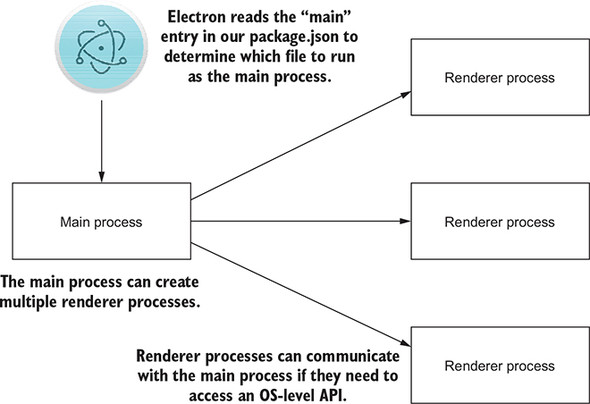
\includegraphics[width=0.4\textwidth]{images/electron-model}
    \caption[Bla]{Multi-process Model Electron from~\cite[Fig. 1.7]{electron-in-action}}
    \label{fig:electron:model}
\end{figure}
\begin{description}
    \item[\textbf{Main}:] \hfill \\ This is the main entry point of the application and responsible for lifecycle management like starting or quitting the app.
    The \texttt{main} process uses so called \texttt{BrowserWindow} module to create and manage each \texttt{renderer} process which is loading web pages into it.
    Since only the \texttt{main} process is running inside a Node.js environment, it is the sole part of the application that can import Node.js modules using \texttt{require}.
    This forces each \texttt{renderer} process to interact with the \texttt{main} process if they want to consume system \ac{API}s for purposes like saving files or opening dialogs~\cite{ElectronDoc,electron-in-action}.

    \item[\textbf{Renderer}:] \hfill \\ A \texttt{renderer} process is responsible for rendering web content by loading web pages into it and presenting them to the at the browser window.
    Additionally, JavaScript code can be loaded and executed inside a process.
    Each \texttt{renderer} process can be created or destroyed by the main process using the \texttt{BrowserWindow} module as mentioned before.
    This leads to the fact, that \texttt{renderer} processes are isolated from each other following the Chromium principles of a multiprocess model and is reasoned by limited affection of
    faulty or malicious code on the entire app.
    The \texttt{renderer} processes are only able to communicate between each other indirectly via the \texttt{main} process or by using \texttt{MessagePorts}.
    This is called \ac{IPC}~\cite{ElectronDoc,electron-in-action}.
\end{description}

\subsubsection{Inter Process Communication}
As mentioned above \texttt{main} and \texttt{renderer} processes are only able to communicate using \ac{IPC}.
\begin{figure}[ht]
    \centering
    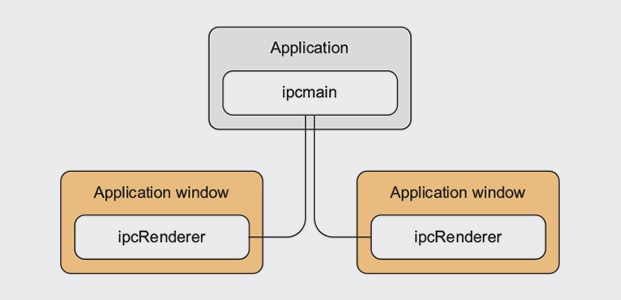
\includegraphics[width=0.4\textwidth]{images/ipcElectron}
    \caption[Bla]{IPC Communication of Electron~\cite[Fig. 6.5]{electron-nwjs}}
    \label{fig:electron:ipc}
\end{figure}
Therefore, Electron provides two modules, one for the \texttt{main} process, called \texttt{ipcMain} and one for \texttt{renderer} process, called \texttt{ipcRender}.
\figref{fig:electron:ipc} points out the process of exchanging data between two or more processes.
Both of them are Node.js \texttt{eventEmitter} modules and capable of executing asynchronously and synchronously communication either uni- or bidirectional.
It should be noticed, that this kind of \ac{IPC} communication is only for \texttt{renderer} to \texttt{main} and vice versa, which can be seen in \figref{fig:electron:ipc}.
A communication between different \texttt{renderer} processes can be archived either indirectly using the \texttt{main} process or directly with \texttt{MessagePorts}.
The advantage of using the direct variant is, that the workload of the \texttt{main} process can be reduced by using a new, hidden \texttt{renderer} process, which serves as a worker for the web content \texttt{renderer}.
A \texttt{MessagePort} can be seen as a communication channel between two \texttt{renderer} processes.
It is once defined inside the \texttt{main} process which informs the \texttt{renderer} processes about belonging \texttt{MessagePorts} from other processes and establishes the connection.
After that, the actual communication does not rely on the \texttt{main} process anymore.
This will reduce workload for the \texttt{main} process in case of message forwarding as well as outsourcing heavy workloads to worker processes~\cite{ElectronDoc}.
\subsubsection{Context Isolation}
Electrons multiprocess model also intends distinct purposes for each process.
As described before only the \texttt{main} process has access to node modules.
In contrast to that only the \texttt{renderer} process has access to \ac{HTML} \ac{DOM}s.
Since using just \ac{IPC} represents a major security issue, Electron introduced a feature called \textbf{Context Isolation}.
This splits the logic of a \texttt{renderer} process into two different contexts.
On the one hand the \texttt{renderer} process as already described and on the other a so called \texttt{preload script}.
The \texttt{preload script} is attached to the \texttt{main} process at the creation of the \texttt{BrowserWindow} module.
It has access to both node modules and \ac{HTML} \ac{DOM}s at its own context and will be executed before the \texttt{renderer} process loads the web page into it.
Although the \texttt{preload script} and the \texttt{renderer} process do both own a window object, which provides the displayed browser window, it is not the same object since they are both running at
different contexts.
The \texttt{preload script} consists of a \texttt{contextBridge} module which is responsible for safely exposing selected properties of the \texttt{main} process to the \texttt{renderer} and vice versa.
Inside this module an \ac{API} can be defined for providing access with \ac{IPC} objects to resources of different processes~\cite{ElectronDoc}.

\subsection{Frontend}
\label{subsec:electron:frontend}
The frontend part of an electron-based app consists of the chromium content module and provides all the core features that are required to render \ac{HTML} content
or access Web-\ac{API}s.
It is important to notice, that the content module is not equal to the chrome web-browser since the chrome web-browser wraps around the content module, but provides
several features, the content module does not provide, like managing bookmarks, spellchecking, safe-browsing or securely saving passwords.
The content module itself includes two parts.
A browser engine called \textbf{Blink} and a JavaScript engine called \textbf{V8}~\cite{electron-in-action}.
\begin{description}
    \item[\textbf{Blink}:] \hfill \\ Blink serves as a browser engine inside the chrome content module and therefore is responsible for translating \ac{HTML} documents to the actual view, a user gets presented.
    Originally chromium used webkit as browser engine, which was developed and maintained by Apple, but fundamental disagreements between Apple with its restricted policy and Google led to the fact,
    that Google forked the webkit engine and uses it as a grounding for their own engine~\cite{heiseBlink,blinkGoogle}.
    It relies on the same architecture as mentioned in~\ref{subsec:electron:architecture}, whereas blink is running inside a \texttt{renderer} process and uses one main thread
    and multiple worker threads that do the layout calculations.
    \item [\textbf{V8}:] \hfill \\ V8 is written in C++ and responsible for compiling and executing JavaScript code as well as memory management like allocation or garbage collecting.
    It can be seen as the executing background part of the content module, which transforms JavaScript code into C++ code, which in turn is translated into machine-readable byte-code,
    but it also provides the possibilities for developers to write own C++ applications that can expose their functions to JavaScript code to add new features or improve performance of execution~\cite{V8Doc}.

\end{description}
Summarized the content module provides all features to Electron that are necessary to develop a classical browser application.
But since classical browser applications are restricted by the OS for example in case of file-system access, the use-cases are limited.
This is the reason, Electron has combined the content module with the Node.js runtime.
%each view is rendered at a separate process, called \textbf{renderer}.
%The reason for this is that faulty or malicious code is limited in its affection at the whole app.
%Each process is controlled by a single process, which is also the entry point of the app, called \textbf{main}.

\subsubsection{Backend}
\label{subsec:electron:backend}
%TODO Add more information
As backend for all electron-based applications the Node.js runtime is used.
Node.js is a framework allowing developers to implement server-side applications using JavaScript, and as the chromium content module of~\ref{subsec:electron:frontend} it utilizes the V8 JavaScript engine to execute JavaScript code, but also provides more functionalities like the mentioned filesystem access
or importing external modules.
Furthermore, a package manager, called \ac{NPM}, with ``more than one million packages``\footnote{\url{https://www.npmjs.com/}} is included.
This amount of packages is a result of an increasing popularity Node.js experienced since its release, providing the capabilities to implement a wide-range of applications.
The reason for utilizing Node.js runtime as a backend for all Electron applications is its privileges.
At traditional web-applications, the client-side is restricted through the OS to consume or request data from a third party \ac{API}\@.
Because of that, the client has to request the server, which then is consuming the third party \ac{API}\@.
Since Node.js has these privileges, the detour at the server-side falls away, guaranteeing electron applications these accesses at the client side~\cite{electron-in-action, electron-nwjs}.



    %Tauri checked
    \section{Tauri}
\label{sec:tauri}
Tauri was first released at \displaydate{dateTauriRelease}~\cite{tauriRelease} and downloaded approx. $58\,000$ times\footnote{According to \url{https://npm-stat.com/charts.html?package=tauri&from=2019-12-31&to=2022-08-12}}.
It resulted as discontent of Electron from the Tauri developers especially in case of resource consumption and security due to uncontrollable dependencies~\cite{tauri}.
They criticized the enormous resource consumption even of the simplest applications as well as the fact, that Electron does not have control over their dependencies.
If Chromium encounters a zero-day-exploit and releases a patch, Electron has to include this patch and also release a newer versions.
This leads to the fact, that users of an Electron-based application have to update their Electron version to close this security issue.
This timespan, between first fix of chromium and the users update of the application, is a high vulnerability against potential attackers.
In this regard, the developers also criticized the power of the privileges Electron applications have, allowing attackers to have access to the entire hard drive of the user for example~\cite{tauri}.
But like Electron Tauri experienced increased attention kept in mind that the first stable version has been released this year, which as in~\ref{sec:electron} can be expressed numerically based on GitHub Statistics~\cite{GithubTauri}: \\ \\
\begin{tabular} {| c | c | c | c | c |}
    \label{tab:tauri:statistics}
    Stars      & Forks     & Watching & Used by    & Contributors \\ \hline
    $48\,200$ & $1\,200$ & $403$ & $3\,200$ & $182$
\end{tabular} \\ \\
But unlike Electron, Tauri uses the self developed core, called Tauri, which is written in Rust in combination with WRY, which serves as the rendering library.


\subsection{Architecture}
\label{subsec:tauri:architecture}
The architecture of Tauri is very similar to Electrons multiprocess model.
Tauri also relies on a main process, called \textbf{core} process and multiple rendering processes, called \textbf{webview} for performance as well as security reasons.
\figref{fig:tauri:model} shows the basic architecture of Tauris multiprocess model whereas each \texttt{webview} process is managed by the \texttt{core} process.
\begin{figure}[ht]
    \centering
    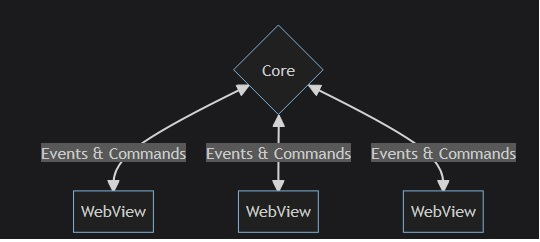
\includegraphics[width=0.4\textwidth]{images/TauriArchitecture}
    \caption{Multi-process Model Tauri from~\cite{tauri}}
    \label{fig:tauri:model}
\end{figure}

\begin{description}
    \item[\textbf{Core}:] \hfill \\ This is the main entry point of the application and the only place where full access to the operating system is provided.
    The \texttt{core} process uses this privileges to create and manage the windows the application.
    But it is also the only point, where the communication between processes is going through, allowing the core process to manipulate or observe \ac{IPC} messages.
    Unlike Electron \texttt{webview} processes are not able to communicate directly between each other, increasing the security since each message has to pass the main process and
    can be discarded if suspicious or unwanted calls are made.
    Additional the \texttt{core} process is responsible for global scoped cases such as database access or managing application or \ac{OS}-specific settings that affect the windows.
    Summarized it serves as a centralized management and control point, where the application as itself is maintained and sensitive data is kept to be hidden from the \texttt{webview} processes~\cite{tauri}.


    \item[\textbf{WebView}:] \hfill \\ A \texttt{webview} process renders the \ac{HTML} content of an application using the WebView libraries of the current \ac{OS}.
    Since this library is not included into the final executable but linked at runtime, it differs depending on the operating system the application is running.
    This reduces the size of the executable since the part where the actual rendering takes places is shifted from the application to the operating system but also results
    that developers have to keep in mind the different operating systems~\cite{tauri}.

\end{description}

\subsubsection{Inter Process Communication}
For communication between different processes Tauri also uses Inter Process Communication similar to Electron.
\begin{figure}[ht]
    \centering
    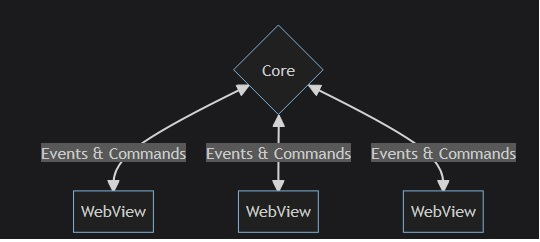
\includegraphics[width=0.4\textwidth]{images/TauriArchitecture}
    \caption{IPC of Tauri~\cite[Figure 1-3]{tauri}}
    \label{fig:tauri:ipc}
\end{figure}
In contrast, Tauri forces developers from the beginning to use the \ac{AMP} paradigm, whereas Electron released this feature at version 14 and only recommends it.
The main advantage of \ac{AMP} is, that direct function access is denied and thus all communication has to pass the \texttt{core} process.
Since it is able to observe the content of messages, it can decide which message will be forwarded and which will be blocked like malicious requests.
Communication can be either unidirectional using events, which can be emitted by both \texttt{core} and \texttt{webview} processes to inform the event recipient but without any response,
or using commands which are bidirectional \ac{IPC} messages but can only be emitted by the \texttt{webview} processes to invoke functions that require access to the operating system like it is shown in \figref{fig:tauri:ipc}.
The core process itself is not able to emit commands to the frontend preventing potential malicious code segments of the core affecting the \texttt{webview} processes~\cite{tauri}.

\subsubsection{Context Isolation}
In contrast to Electron Tauri uses different patterns for isolating communication between the \texttt{webview} processes and the \texttt{core} process and potential critical \ac{API} calls.
They are called Brownfield and Isolation Pattern, whereas the default pattern, that can be configured inside the \texttt{tauri.conf.json} is the Brownfield pattern
\begin{description}
    \item[\textbf{Brownfield Pattern}:] \hfill \\
    The Brownfield pattern can be seen as a design pattern to ensure interoperability between new implemented and existing software.
    This pattern does not categorize software as legacy software but as current state of the art and software developed following this pattern tries to coexist and consider existing software as much as possible.
    This requires a deep knowledge of the existing software and also can result in re-developing significant parts of the existing software when tried to enhance new features.
    Tauri uses this pattern as standard and explains that it tries to be as compatible as possible.
    But unfortunately Tauri does not explain in detail how they are implementing this pattern and how this helps to avoid malicious frontend calls to the Tauri core~\cite{tauri}.
    \item[\textbf{Isolation Pattern}:] \hfill \\
    The Isolation Pattern can be seen as an interposed instance between the \ac{IPC} handler and the processes.
    This instance is providing a sandbox, called Isolation application, which is trusted and secure JavaScript code embedded into an \texttt{<iframe>}.
    The \ac{IPC} handler passes its message to the Isolation application, where it is executed and may be modified or verified.
    After that it will be encrypted, passed back to the \ac{IPC} handler and forwarded to the \texttt{core} process, where it will be handled as normal~\cite{tauri}.


\end{description}

\begin{figure}[ht]
    \centering
    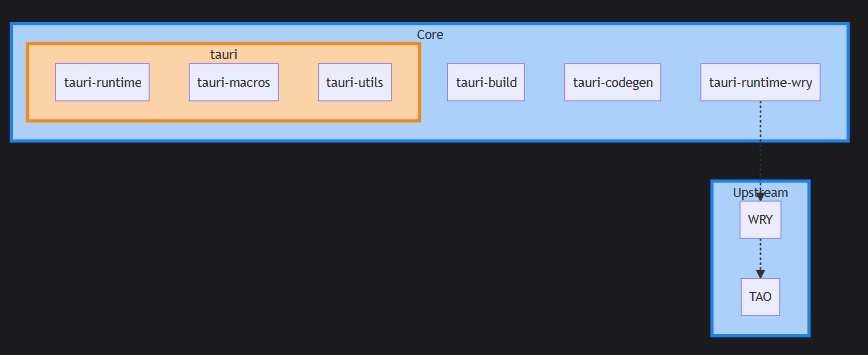
\includegraphics[width=0.4\textwidth]{images/TauriCore}
    \caption{Core Ecosystem from~\cite{tauri}}
    \label{fig:tauri:core}
\end{figure}
As it can be seen in \figref{fig:tauri:core} Tauri splits its framework into two main components.
The Core, containing several modules providing \ac{API} access, utilities and the runtime.
The Upstream containing the two self-developed Rust crates WRY and TAO which are providing libraries for creating browser windows and rendering the WebView and its content.
%Same as described for Tauri.Ref to introduction\ref{subsec:electron:arch}

\subsection{Frontend}
\label{subsec:tauri:frontend}
As mentioned above, Tauri's frontend relies on its own implementation of WebView instead of the entire chromium content module for rendering \ac{HTML} content.
This makes it much smaller than electron applications since their libraries WRY and TAO are using the exising web engines of the three major operating systems Linux, macOS and Windows instead of shipping an entire browser.
\begin{description}
    \item[\textbf{TAO}:] \hfill \\
    TAO is a cross-platform library written in Rust and used for creating and managing application windows.
    It was forked from the Rust crate \texttt{winit} since the developers wanted to enhance more desktop features than the original crate, like menu bars or a system tray.
    This library ships with an entire event loop that can be emitted by windows like resizing or key interactions and is included at the second frontend library WRY\@.
    \item[\textbf{WRY}:] \hfill \\
    WRY is the main library at Tauri applications and responsible for rendering the content of the os-specific web view and based on the webview library~\cite{githubWebview}.
    It acts as an interface between the Tauri core with its low level webview drivers and the webview technology of the current operating system, providing a unique abstraction layer for rendering \ac{HTML} content.
    Since it re-exports TAO and its event loop to guarantee access to \ac{OS}-specific web engines the appearance of the same application may differ on each operating system, depending on the underlying web engine.
\end{description}
%WRY and TAO
%Webview implementierung
\subsection{Backend}
\label{subsec:tauri:backend}
The backend or core of Tauri contains several components, whereas some of them are summarized and called \texttt{tauri} to emphasize the main part of each Tauri application including runtime or the Tauri \ac{API}.
The decision to write the entire backend in Rust was made because of the ownership feature in Rust which provides a set of rules for memory management and avoiding a garbage collector like Java or explicit memory allocation like C~\cite{tauri}.
It can be seen as an approach of trying to be more comfortable for the developer as an explicit allocation but also to force the developer to consider his/her memory handling to implement an efficient application~\cite{klabnik2019rust}.
This set of rules is checked at compile time and if one of them is violated, the program will not compile.
Beside the \texttt{tauri} components there are also additional components included by the core like system-level interactions for the upstream crate WRY .
One of the major advantages of using Rust for the Tauri backend is as already mentioned its ownership rules, avoiding security issues but also the execution time of Rust code which was intended to obtain a similar performance as C++~\cite{klabnik2019rust}.
Furthermore, Rust experienced a significant attention resulting in the adoption of it by big companies like Google or Facebook which assumes an increasing position.


    %Implementation checked
    \section{Implementation of a counter \\ application}
\label{sec:implementation}
As already mentioned at~\ref{subsec:motivation} this section describes the underlying work for this paper and will guide through the entire development process of Electron and Desktop applications.
To obtain comparable results, the methodology of comparison will be explained shortly.
For this paper a basic counter application has been implemented in both Electron and Tauri using just bare \ac{HTML},\ac{CSS} and JavaScript, although both frameworks are supporting most common frontend frameworks like Angular, React or Vue.js.
This decision was made because the paper focuses on presenting the differences and similarities of each framework to the reader and thus using complete frameworks will both blow up the entire application and not concentrate on the essentials.
The counter application consists of a simple Counter which is displayed and two buttons providing the possibility to increment or decrement the counter.
Both buttons will have an event listener, that sends \ac{IPC} messages to the backend and as response get the new calculated counter value which then will be displayed to show the entire communication chain of each framework.
Therefore, each application will contain the same \ac{HTML} content as it can be seen in \figref, that is displayed and only the API calls of the frameworks will differ, depending on their architecture.
To avoid unnecessary distortion of measurements only the fundamentals of each framework are included without any additional helper libraries for better styling or further functionalities.

%This section will include a short explanation of the counter app as an example application.
%It will show the features and define the requirements for an objective comparison.

\subsection{Methodology}
\label{subsec:method}
For benchmarking the applications in case of build time GitHub Actions are used.
Thus, each project has its own GitHub repository with a workflow.yaml defining the actions' workflow.
Each Action will run on the three major operating systems macOS, Windows and Linux, set the prerequisites for the framework respectively and use the recommended build tool, \texttt{electron-forge} for Electron and the \texttt{tauri build} command for Tauri.
This will result in three jobs for each project, whereas the build time for each framework on each os will be measured, since usual prerequisites are installed once and thus not measured.
Time of execution is measured using hyperfine\footnote{\url{https://github.com/sharkdp/hyperfine}} which is a command line benchmark tool.
Therefore, the executable of each framework will be started by command line, with hyperfine switched in front.
To see the difference between a cached and uncached execution, the first run does not have any warmup actions and so prevent the operating system from loading the application into the filesystem cache.
This results in following command \shellcmd{hyperfine --runs 10 --warmup 2 'start <executable>}
To gather meaningful data, hyperfine will run 10 instances of the executable to obtain a min-max range as well as a mean execution time.

For memory consumption the python library memory-profiler\footnote{\url{https://pypi.org/project/memory-profiler/}} will measure the memory consumption of each executable over a timespan of 60 seconds,
enough to get from startup to idle state.
This timespan will be set to 60 seconds, to allow interaction with the application as well as complete startup and idle state.
Since the applications rely on multiprocess models and may also spawn children, these are recorded too, to gather trustful memory consumption measurements.
To archive this measurement following memory profiler command is used \shellcmd{mprof run --include-children --multiprocess --timeout 60 <executable>}
It is important to notice that Tauri comes with a single executable file, whereas Electron ships with an installer which has to be executed first in order to get the actual executable application running.
All Electron measurements will use this installed executable as foundation.

Except build time for different operating systems which will use GitHub Actions, the measurements of execution time, memory consumption or binary size
are made with Windows 11.
The implemented application is based on Electron Version 19 the newest stable release at time of writing this paper respectively Tauri version 1.0.2.

%This subection section will take the findings of~\ref{sec:electron} into action and analyze the development and building process as well as the performance of the executable application.

\subsection{Development}
\label{subsec:impl:dev}
The development process is following the best practices section of each framework~\cite{ElectronDoc,tauri} to avoid deprecated or inefficient calls.
Implementation is done with usage of Visual Studio Code, a common, lightweight \ac{IDE} commonly used for web development and also recommended by both Electron and Tauri.

\subsubsection{Prerequisites}

Since Electron mainly relies on Node.js, this as well as the actual Electron framework are the only dependencies that are needed to start developing.
It should be noticed, that Electron is installed as dev dependency since packaged applications are shipped with an Electron binary and therefore are not needed to be defined as production dependency.
Although they are not used, since the application is based on just \ac{HTML} \ac{CSS} and JavaScript, Electron provides several tools for generating a project with fundamental boilerplate code for most common web frameworks like Angular or React.\\
Tauri in contrast needs several more prerequisites to start developing which includes WebView2, the actual web engine for Windows that is used by Tauri as well as Rust, what on the other hand pre-conditions Microsoft Visual Studio C++ Build tools.
Since Tauri consists of two subprojects, the Rust Core and the Frontend it provides a tool for scaffolding boilerplate projects using the most common web-frameworks as well as just plain \ac{HTML} \ac{CSS} and JavaScript (called Vanilla.js by Tauri),
whereas Node.js as prerequisite is implied too.
To initiate the Rust project, once the entire project is scaffolded, the CLI module of tauri needed.
This tool will generate a minimal Rust project set-up to use Tauri with the selected web-framework and specify the location of all the belonging web assets.

Once each project is initialized a basic \ac{HTML} file combined with basic \ac{CSS} styling is created to specify the actual appearance of the application.
The main JavaScript file of the frontend is specified inside the \texttt{package.json} of each framework.
As mentioned before, two buttons will be added to increment or decrement the counter for presenting a basic \ac{IPC}.
Therefore, each button has an event listener which will listen to click events and call the appropriate \ac{IPC} chain.

\subsubsection{Implementation - Electron}
\label{subsubsec:impl:electron}
Following best practices the Electron framework is divided into three JavaScript files, whereas the main process \\(\texttt{electron.js}) represents core process as described in section~\ref{subsec:electron:architecture}.
This file contains the actual browser creation which will spawn a new renderer process  with the corresponding preload script as well as specifications of the content that should be loaded inside the window.
But also required handlers of the \texttt{ipcMain} module including the logic are implemented here.
The second JavaScript is the preload script that contains the \texttt{contextBridge}  and \texttt{ipcRenderer} modules of Electron and exposes the API to the renderer process.
This preload script is linked to the main process at the definition of the browser window, that is created by the \texttt{electron.js} file.
The third JavaScript file is the renderer script, that is responsible for adding basic interaction processing that can occur.
\newpage
\begin{lstlisting}[language=JavaScript,label={lst:rendererjs}, caption={Excerpt of render.js}]
inc_btn.addEventListener('click', async () => {
    counter.innerText =
        await window.electronApi.increment(document.getElementById('counter').innerText)
})
\end{lstlisting}
\begin{lstlisting}[language=JavaScript,label={lst:preloadjs}, caption={Excerpt of preload.js}]
contextBridge.exposeInMainWorld('electronApi', {
    increment: (param) => ipcRenderer.invoke('incrementChannel', param)
})
\end{lstlisting}
\begin{lstlisting}[language=JavaScript,label={lst:electronjs}, caption={Excerpt of electron.js}]
ipcMain.handle('incrementChannel', async(param) => {
    return parseInt(param) + 1;
})
\end{lstlisting}

Once a button is pressed a click event will be emitted and the code shown at listing~\ref{lst:rendererjs} will be executed.
Inside the event listener the related function of the \ac{API}, that is exposed by the preload script and shown at listing~\ref{lst:preloadjs}, will be called.
This will invoke the \texttt{ipcRenderer} module which takes the params of the \texttt{increment} function and send a message using the defined channel, at this case \texttt{incrementChannel} and wait for the response of the handler of the
\texttt{ipcMain} module at listing~\ref{lst:electronjs}.
Since the handler is inside the \texttt{electron.js} which is the main process of the application, this is the place where node modules can be imported and thus the only way for renderer process to use them.
The handler will return the new calculated passed parameter back to the \texttt{ipcRenderer} which then will be set as new counter value as it can be seen at listing~\ref{lst:rendererjs}.
Addressing the difficulty of implementing an application with Electron is has to be said that the entire app can be written with JavaScript,\ac{HTML} and \ac{CSS} which may have a great impact
on small teams of web-developers that are already familiar with those web technologies.
The framework itself is well documented including examples that cover of most use cases and constantly updated to follow the recommendations of the newest releases by the maintainers.
Since Electron uses Node.js as runtime it benefits from its huge community providing libraries for almost any scenario.
Nevertheless, since Electron has released up to 19 stable release versions, there has changed a lot over the years, causing developers to update their applications constantly, which in worst case could result
in reimplementing the entire process communication to migrate their codebase.
\subsubsection{Implementation - Tauri}
Once the two subprojects of the Tauri application are initialized the same frontend as described in section~\ref{subsubsec:impl:electron} will be added to the specified web assets folder,
containg the \ac{HTML} file, a \ac{CSS} stylesheet as well as the JavaScript file for processing interaction events, at this example the EventListener of both buttons.

\begin{lstlisting}[language=JavaScript,label={lst:indexjsTauri}, caption={Excerpt of index.js}]
incBtn.addEventListener('click', function() {
    invoke('inc', {cnt: parseInt(counter.innerText)}).then((response) => counter.innerText=response)
})
\end{lstlisting}

\begin{lstlisting}[language=Rust,label={lst:mainrsTauri}, caption={Excerpt of main.rs}]
#[tauri::command]
fn inc(mut cnt: i32) -> String {
  cnt+=1;
   return cnt.to_string();
}

fn main() {
  tauri::Builder::default()
    .invoke_handler(tauri::generate_handler![inc])
    .run(tauri::generate_context!())
    .expect("error while running tauri application");
}
\end{lstlisting}
The core process as described in section~\ref{subsec:tauri:architecture} is created by the \texttt{main.rs} file of the Rust project inside the main function of listing~\ref{lst:mainrsTauri}.
Inside the main method the default method of Tauris Builder structure is executed which will set WRY as runtime for the application.
The \texttt{invoke\_handler} method will set up the passed handlers of the application that will be responsible for \ac{IPC}.
Inside the \texttt{run} method, that will execute the passed context, the actual context is generated by the \texttt{generate\_context} method, that will read the config file, which is the \texttt{tauri.conf.json} by default and create the context of the application.
To indicate handlers that will be executed once the fronted makes an \ac{IPC} request to the core, Tauri uses the \texttt{\#[tauri::command]} makro for commands and \texttt{\#[tauri::event]} for events respectively.
As it can be seen at listing~\ref{lst:indexjsTauri} once a button is pressed, the implemented event handler will be called. 
This will call the \texttt{invoke} method of the Tauri \ac{API} which can either be imported as npm package or set to global inside the config file.
The method takes two parameters whereas the first defines the name the command that should be executed, similar to the channels of Electron and the second parameter is containing all data that should
be passed to the command method and is returning a promise which then can be processed.
Since Tauri is using a protocol similar to \ac{JSON-RPC} the passed data has to serializable.
After the \ac{IPC} request has reached the core, the corresponding method will be executed which can be seen in listing~\ref{lst:mainrsTauri}.
The command takes integer as parameter, increments it and then returns a string, that will be wrapped into a promise.
After the invoke method returned the promise which contains the processed data of type string it will update the counter.
Referring the complexity and difficulty the reader should keep in mind that implementing a Tauri application nowadays requires knowledge with Rust, since the backend and therefore the process communication can only be implemented in Rust.
Although the Tauri developers announced plans to provide the support of different languages for the backend at the time, this paper is written, Tauri only supports Rust as backend language.
The documentation of Tauri tries to follow the same schema as Electron but is often indistinct and ambiguous or does not provide any detailed information of subjects.
Especially the choice of using Rust as backend cuts limits the provided libraries to those of Rusts package manager cargo which limits the amount of usable libraries in contrast to Node.js and may result in writing
own functionalities since.
%As mentioned at~\ref{subsec:electron:architecture} the main process of Electron is running inside the Node.js environment, meaning that this is the only place where Node-Modules can be \textbf{required} and used.
%At this subsubsection the general development process of an Electron application is discussed but also the actual development using the screencast
%application as an example.
%Are there any templates provided, which dependencies and tools are needed for implemention, debbuging and testing.
%Are they already provided by the installer?
%Also have a short look at the documentation e.g.are there any guides, community feedback.

\subsection{Performance}
\label{subsec:impl:performance}
Once the applications are implemented the build process of each framework is invoked to create an executable which is the foundation of performance measurements.
The build time for each application is measured using GitHub actions, whereas it has to be mentioned, that this will be done on completely bare metal runners, that did not cache anything to obtain more comparable measurements
since each framework may cache at different scales.
After the executables are created the performance of both are measured using the techniques described in section~\ref{subsec:method}.

\subsubsection{Build Time}
\label{subsubsec:perf:buildtime}
Table~\ref{table:buildingtime} summarizes the results of the GitHub Actions for each operating system and the binary size.
It is clearly visible that building a Tauri app requires much more time than Electron applications spread over the operating systems.
This can be explained with the complex process of Rust compilation like incremental compilation techniques or time-consuming code analysis~\cite{rustCompileTime} combined with the absence
of caching since the GitHub Actions were executed on bare-metal systems.
This owed due the fact of providing comparable results and may not occur at every-day development where applications are build constantly to test features and therefore cached to reduce compile time.
\\
\begin{tabular} {| c | c | c | c | c |}
    \hline
    \multicolumn{4}{|c|}{Building time in seconds} & \\ \hline
    Framework & \multicolumn{3}{|c|}{Operating System} & Size [KB]  \\ \hline
    & Windows & Ubuntu & MacOS &  \\ \hline
    Tauri & 863 & 616 & 389 & $6\,924$  \\ \hline
    Electron & 115 & 121 & 44 & $145\,361$ \\ \hline
\end{tabular}
\label{table:buildingtime}
\\ \\

The binary size of the compiled executable amounts to $6\,924$ for the Tauri application respectively $145\,361$ for Electron which is direct result of the architecture of both framework as mentioned in sections~\ref{subsec:electron:frontend} and~\ref{subsec:tauri:frontend}.
Electron ships the executable with an entire web browser making whereas Tauri makes use of the system specific web engine and therefore is able to reduce its size by a factor of approximately 21.
This may be an advantage or disadvantage depending on the developers or customers point of view, since the different web engines of each system may result in slightly different appearances of the application.

\subsubsection{Memory Consumption}
\label{subsubsec:perf:memory}
\figref{fig:electron:memory} and \figref{fig:tauri:memory} show the entire memory usage of the implemented applications including their child processes.
Although the Electron application consumes more memory at startup, causing a peak of approximately 400 MiB at \figref{fig:electron:memory} it decreases its memory consumption up to approximately 290 MiB,
whereas the Tauri Application is constantly at a consumption of roughly 320 to 330 MiB\@.
Both figures also point out that Tauri has more processes involved into the application than Electron.
Those graphics stay in contrast to the actual benchmarks provided by Tauri\footnote{\url{https://tauri.app/about/benchmarks/}} and thus only the benchmarks for Electron are made public it is not possible to explain the discrepancies between both frameworks objectively.
\begin{figure}[ht]
    \centering
    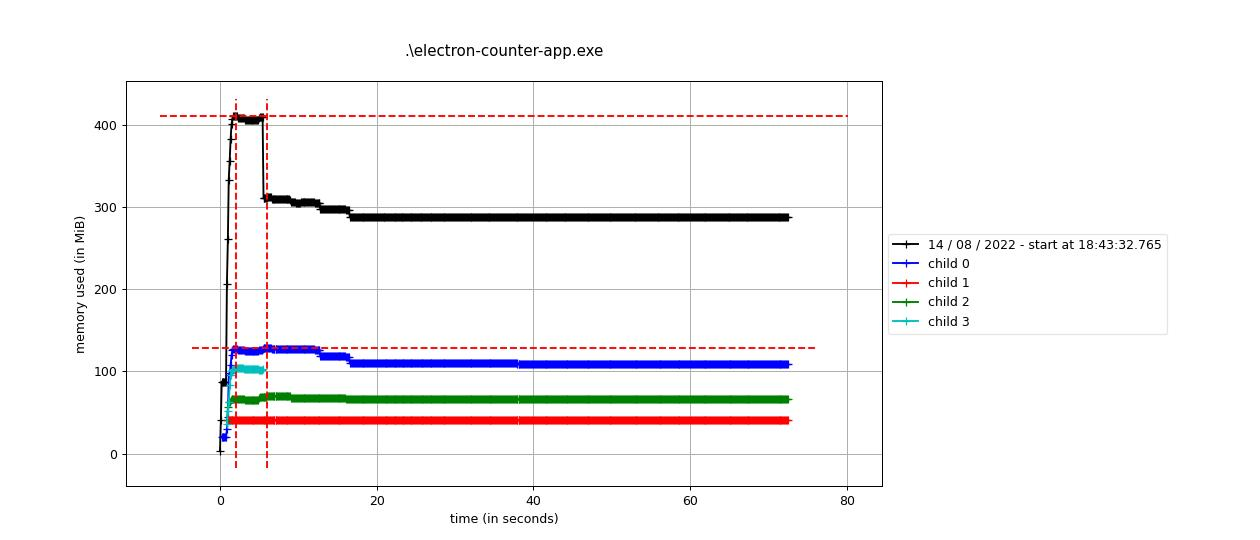
\includegraphics[width=0.5\textwidth]{images/ElectronMemCons}
    \caption[]{Memory consumption of Electron executable obtained from memory profiler}
    \label{fig:electron:memory}
\end{figure}
\begin{figure}[ht]
    \centering
    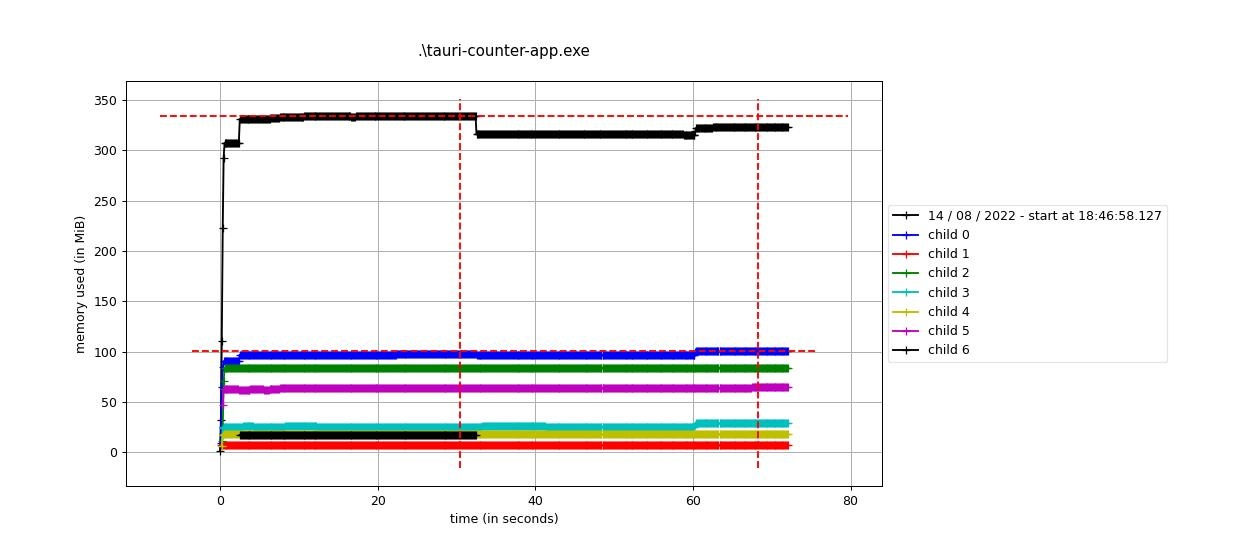
\includegraphics[width=0.5\textwidth]{images/TauriMemCons}
    \caption[]{Memory consumption of Tauri executable obtained from memory profiler}
    \label{fig:tauri:memory}
\end{figure}
\\
\subsubsection{Execution Time}
\label{subsubsec:perf:execution}

The measurements of \texttt{hyperfine} are shown below, whereas the mean values include their standard deviation based on ten measurements and caching describes the warmup option that is added to the second run of hyperfine.
The high standard deviation of both table~\ref{table:exec:electron} and table~\ref{table:exec:tauri} at the \textbf{Without caching} row can be explained with the max values of the same row.
The max value is more than 2 standard deviations away from the mean value meaning it is not a probable execution time, but it also shows the effect of filesystems caching.
To obtain more reliable and undistorted measurements the warmup option of hyperfine showed the results of execution time after the application is cached.
Both tables point out, that execution time of the Tauri application is faster than the Electron application at all measured values even if the mean values of Electron and Tauri only slightly differ.
This is reasoned by Tauri's usage of Rust as backend which has a performance similar to C++~\cite{rustPerformance} and thus is more performant than JavaScript~\cite{C++Javascript}.

\begin{tabular} {| c | c | c | c |}
    \hline
    \multicolumn{4}{|c|}{Execution time of Electron [ms]} \\ \hline
     \multicolumn{4}{|c|}{}\\ \hline
     & Mean   & Min & Max     \\ \hline
    Without caching & 17.3 $\pm$ 23.3 & 6.5 & 82.9  \\ \hline
    With caching & 18.0 $\pm$ 14.8 & 7.5 & 49.6 \\ \hline
\end{tabular}
\label{table:exec:electron}
\\ \\

\begin{tabular} {| c | c | c | c |}
    \hline
    \multicolumn{4}{|c|}{Execution time of Tauri [ms]} \\ \hline
    \multicolumn{4}{|c|}{}\\ \hline
    & Mean & Min & Max     \\ \hline
    Without caching & 17.1 $\pm$ 10.5 & 5.8 & 35.4  \\ \hline
    With caching & 15.1 $\pm$ 7.9 & 5.2 & 29.0 \\ \hline
\end{tabular}
\label{table:exec:tauri}
\\ \\
%At this subsubsection the actual performance of the example application is analyzed.
%Memory consumption, known security issues, bugs, freezes etc.
%This subsection section will take the findings of~\ref{sec:tauri} into action and analyze
%the development and building process as well as the performance of the executable application.

    \section{Summary}
\label{sec:summary}
This section will take the knowledge of \ref{sec:electron} and \ref{sec:tauri} as well as the analysis of \ref{sec:implementation} to contrast them.

\subsection{Differences}\label{subsec:differences}
This subsection will work out the differences between the two frameworks
with regard to Architecture, Frontend, Backend, Development, Build and Performance.

\subsection{Similarities}\label{subsec:similarities}
This subsection will work out possible similarities between the two frameworks with regard to Architecture, Frontend, Backend, Development, Build and Performance.
    \section{Conclusion}
\label{sec:conclusion}
%At this section a conclusion is made based on the advantages/disadvantages of each framework
%described in \ref{sec:conclusions}.
%Are there different use-cases for each framework, are they concurrent to each other, etc.?
Reminding the intention of the developers of Tauri mentioned at section~\ref{sec:tauri} and contrasting them to the measurements discussed in section~\ref{sec:implementation}
it can be determined that some aspects like execution time or security of Tauri applications compared to Electron are accurate.
Tauri applications have a more efficient performance in aspects of memory usage or execution time, due to the fact of using Rust as backend core.
Nevertheless, some benchmarks provided by Tauri, especially in case of memory consumption could not be reproduced or investigated further since those are not provided public.
But as mentioned in section~\ref{sec:summary} Tauri compared to Electron does a step towards the traditional web development, where system-specific requirements have to be considered and
therefor at worst case an application for each operating system has to be implemented.
Although this might need only small changes on the entire code base redundant code follows from this.
Tauri has experienced much attention since its first release but at the current state is not suitable for big applications in production mode.
This statement is based on different aspects.
First, the documentation is difficult to understand resulting in paraphrases or one-sentenced explanations of entire architecture aspects like their design patterns, than actual explaining them.
This results in uncertainties how the Tauri framework is doing tasks in detail.
Especially the security section is rather describing possible threats that can occur during development than explaining their implemented solutions or how they affect existing code.
Although documentations do not have to be objective, the Tauri documentation often compares parts of it against Electron applications even if some of them are referencing old and deprecated modules like ASAR files~\cite{tauri}. \\
Second, the knowledge of Rust required to implement more complex applications that need access to the Rust core.
Electron can be written by just using JavaScript and thus lowers the bounds for small web-development teams, since JavaScript is widely used at this branch.
For those teams, implementing a Tauri application will result in learning a complete new programming language and in worst case if they do not have any knowledge in comparable languages like C++
learning complete new programming patterns like \ac{OOP} principles or memory management.
This consumes more resources during the development process and thus will lead to an increasing timespan between the initial development and a release of the application.
Although Tauri has claimed to face this issue and announced to provide a backend that can be written using different languages, it is neither implemented nor scheduled yet.
Several standard web techniques and functions like downloading or native menu items are not implemented too.
This will cause developer teams add new functionalities to their applications since they are not provided by Electron yet.
Third the community itself as well as the support of the developers, since Tauri and especially Rust suffers from a lack of functionalities and Features that are provided Node.js or Electron.
Since Electron is used by many well-known companies like Microsoft with their Teams or Visual Studio applications or Discord and their same named application,
this impacts the interests of improving the framework as well as the popularity for small development teams.

Summarized Tauri improves some problems Electron has to deal with due to its architecture and underlying frontend and backend parts but is not suitable option for implementing applications
that are aimed to be provided to millions of users or small development teams that do not have the resources that are required to implement Tauri applications.
As it was pointed out by the authors of~\cite{explorationstudy} development teams using Electron have median number of 1 core developer.
Using Tauri will result increasing complexity for those core teams although the background of the developers was not determined by the authors depending on the knowledge of system-related programming principles.
Thus, the release time of applications or new features at least at the beginning of projects will shift further.
This could affect developers that or even companies that want to obtain a balanced mix between release intervals and invested resources.
It is a complex framework compared to other common cross-platform web-frameworks for implementing desktop applications but provides the possibility to develop efficient and small-sized applications compared to Electron, although
they are currently limited by the Rust core.


\subsection{Further work}
Since this paper is based one the first stable release of Tauri, the topic has to be observed in the future, especially if the developers are improving their framework and documentation considering the requirements of the community.
This could result in further performance comparisons between both frameworks or the productive operation of applications build with Tauri, especially with applications requiring intensive cpu workload or complex calculations.
It also needs further research or observation how the developers of Electron are dealing with the issues, the Tauri developers have mentioned in the future, including investigation of development that are using Electron if
they want to migrate to Tauri or respectively as well as the reasons for that.
Since Tauri is a framework with a new approach of using a system-related programming language of developing cross-platform desktop applications, further investigation in terms of how this affects establishing Rust especially as web-development language is necessary.
Although the resource consumption of Electron is often criticized, there is no scientific publication how this influences the consumer choice of using those applications, since modern desktop computers do not suffer from a lack of memory in general
or how this affects companies in their decision to migrate from Electron to Tauri.



% macht speicher so einen großen einfluss
    \section{List of Abbreviations}
\label{sec:list-of-abbreviations}
\hfill
\begin{acronym}
    \acro{HTML}[HTML]{Hypertext Markup Language}
\end{acronym}

\begin{acronym}
    \acro{CSS}[CSS]{Cascading Style Sheets}
\end{acronym}

\begin{acronym}
    \acro{API}[API]{Application Programming Interface}
\end{acronym}

\begin{acronym}
    \acro{AMP}[AMP]{Asynchronous Message Passing}
\end{acronym}

\begin{acronym}
    \acro{NPM}[NPM]{Node Package Manager}
\end{acronym}

\begin{acronym}
    \acro{IPC}[IPC]{Inter-Process Communication}
\end{acronym}

\begin{acronym}
    \acro{OS}[OS]{Operating System}
\end{acronym}


\begin{acronym}
    \acro{DOM}[DOM]{Document Object Module}
\end{acronym}

\begin{acronym}
    \acro{IDE}[IDE]{Integrated Development Environment}
\end{acronym}


    \newpage

    \bibliography{main}
    \bibliographystyle{plain}

    \balancecolumns

\end{document}
